\section{Differentialrechnung}
\subsection{Einleitung}
\begin{LA}
    {Weg-Zeit-Diagramme}{}
    Eine Rangierlokomotive bewegt sich entlang der Geleise vor- und rückwärts. 
    \begin{center}
        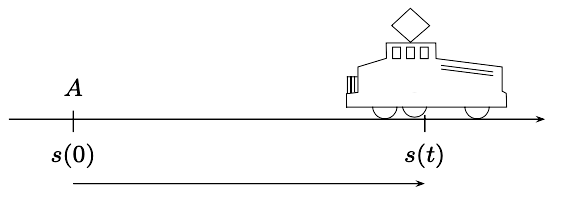
\includegraphics[width=0.25\textwidth]{media/rangierlok.png}
        
    \end{center}
    
    Das folgende „Weg-Zeit-Diagramm“ beschreibt die Bewegung der Lokomotive während 2 Minuten. 
    Auf der horizontalen Achse ist die Zeit in Sekunden dargestellt. Auf der vertikalen Achse ist der Abstand in Metern von einem Bezugspunkt A auf den Geleisen angegeben. Der Zeitpunkt $t=0$ ist der Moment, in welchem die Lok den Punkt A passiert.
    \begin{center}
        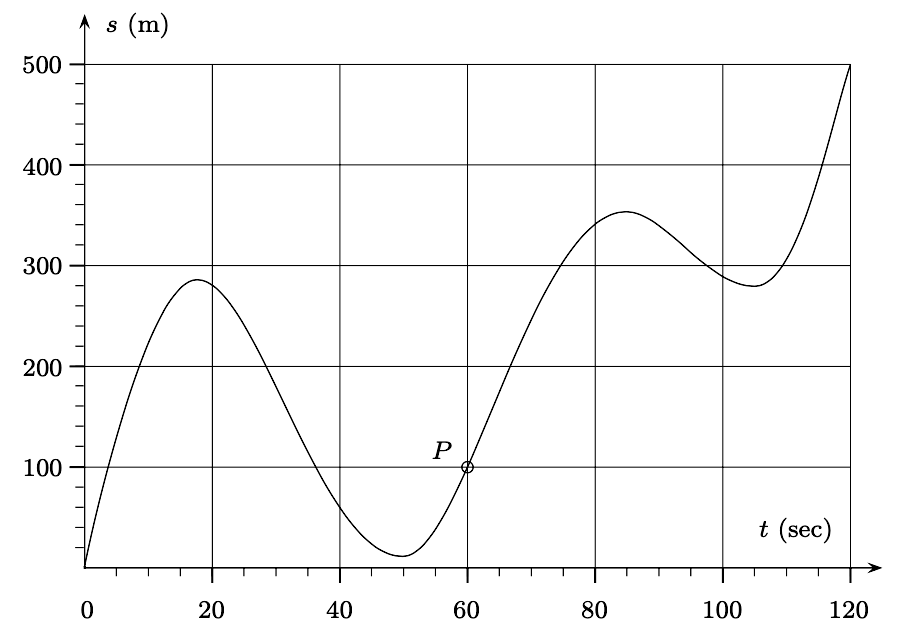
\includegraphics[width=0.6\textwidth]{media/LokWegZeit.png}
    \end{center}
    \begin{enumerate}
        \item Zu welchen Zeitpunkten befindet sich die Lok 200 Meter vom Punkt A entfernt?
        \item In welchen Zeitintervallen fährt die Lok rückwärts?
        \item Nach 60 Sekunden ist die Lok ungefähr 100m vom Punkt A entfernt. Wie viele Meter ungefähr hat sie \textbf{insgesamt} zurückgelegt?
        \item Berechne ungefähr die durchschnittliche Geschwindigkeit der Lok während den ersten 10 Sekunden.
        \item Berechne ungefähr $\frac{s(40)-s(20)}{40-20}$. Was für eine physikalische Bedeutung hat das Resultat und wieso ist es negativ?
        \item Schätze: Wann fährt die Lok am langsamsten? Wann am schnellsten?
    \end{enumerate}

\end{LA}
\clearpage
\begin{LA}
    {Mittlere und momentane Geschwindigkeit}{}
    Auf der 100-Meter-Bahn der KS Im Lee wird ein Roboter getestet. Er wird auf die Startlinie gesetzt und beschleunigt schnell in Richtung Ziellinie. Während der Fahrt folgt die Bewegung des Roboters der Bewegungsgleichung:
\[
    s(t) = \frac{1}{4} t^2
\]
Das bedeutet, dass der Roboter nach $t$ Sekunden die Strecke $s(t) = \frac{1}{4} t^2$ in Metern zurückgelegt hat. Wir denken uns entlang der Bahn ein Messband ausgelegt, sodass wir immer die Position des Roboters in Metern nach dem Startpunkt ablesen können.
\begin{enumerate}
    \item Skizziere den Graphen der Funktion $s(t)$ im Bereich $0 \leq t \leq 8$.

 

\begin{center}
    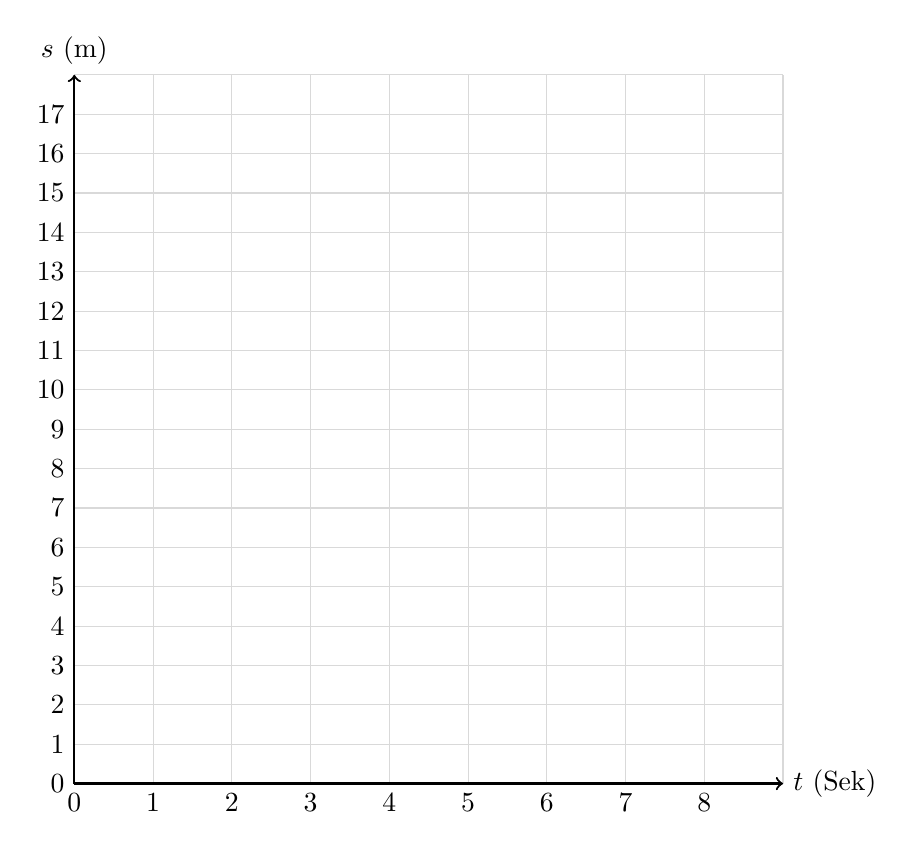
\begin{tikzpicture}
       
        
        % Rasterlinien
        % \draw[gray!30, step=1] (0,0) grid (8,9);
        \draw[gray!30,xstep=1, ystep=0.5] (0,0) grid (9,9);  % X-Richtung (Schrittweite 1)
        %\draw[gray!30,step=0.5,ystep=0.5] (0,0) grid (9,9);  % Y-Richtung (Schrittweite 0.5)
         % Achsen
         \draw[->, thick] (0,0) -- (9,0) node[right] {$t$ (Sek)};
         \draw[->, thick] (0,0) -- (0,9) node[above] {$s$ (m)};
        
        % Beschriftungen der Achsen
        \foreach \x in {0,1,2,3,4,5,6,7,8} {
            \node[below] at (\x,0) {\x };
        }
        \foreach \y in {0,1,2,3,4,5,6,7,8,9,10,11,12,13,14,15,16,17} {
            \node[left] at (0,\y/2) {\y };
        }
    \end{tikzpicture}
\end{center}


    \item Welche Position lesen wir auf dem Messband 2 Sekunden nach dem Start ab? Und welche Position 6 Sekunden nach dem Start? Markiere die entsprechenden Punkte auf dem Graphen.
    \item Welche Distanz legt der Roboter zwischen dem Zeitpunkt $t=2$ und $t=6$ zurück? Wie gross ist demnach die Durchschnittsgeschwindigkeit $\bar{v}$ in m/s zwischen den beiden genannten Zeitpunkten?
    \item Zur Berechnung von $\bar{v}$ haben wir so etwas wie „obsi/vorwärts“ gerechnet. Von welcher Geraden ist $\bar{v}$ die Steigung? Zeichne die Gerade in den Graphen oben ein.
    \item Berechne die Durchschnittsgeschwindigkeit des Roboters zwischen den Zeitpunkten $t=2$ und $t=2+\Delta t$ für $\Delta t=4,3,2,1,0.5$.
    \begin{center}
        \begin{tabular}{p{1.5cm} p{1.5cm} p{1.5cm} p{1.5cm} p{1.5cm} p{1.5cm}}
            \hline
            $\Delta t$ & 4 & 3 & 2 & 1 & 0.5 \\
            \hline
            $\bar{v}$ &  &  & &  &  \\
            \hline
                
        \end{tabular}
    \end{center}
  

    \item Bisher war immer die Rede von einer durchschnittlichen Geschwindigkeit im Intervall $[2,2+\Delta t]$. Wie schnell aber fährt der Roboter genau zum Zeitpunkt $t=2$? Das heisst, schätze seine Momentangeschwindigkeit $v(2)$.
    \item Von welcher Geraden ist $v(2)$ die Steigung? Zeichne die Gerade in den Graphen oben.
    \item Was ist die Momentangeschwindigkeit des Roboters zum Zeitpunkt $t=8$?
\end{enumerate}



\end{LA}

\begin{LA}
    {Temperaturverlauf im Ofen}{}
    Während den zehn Minuten, in denen ein Ofen auf 200°C erhitzt wird, verläuft die Temperatur nach der Gleichung:
\[
    T(t) = -\frac{9}{5} (t-10)^2 + 200
\]
wobei $t$ die Zeit in Minuten und $T$ die Temperatur in °C angibt.

\begin{center}
    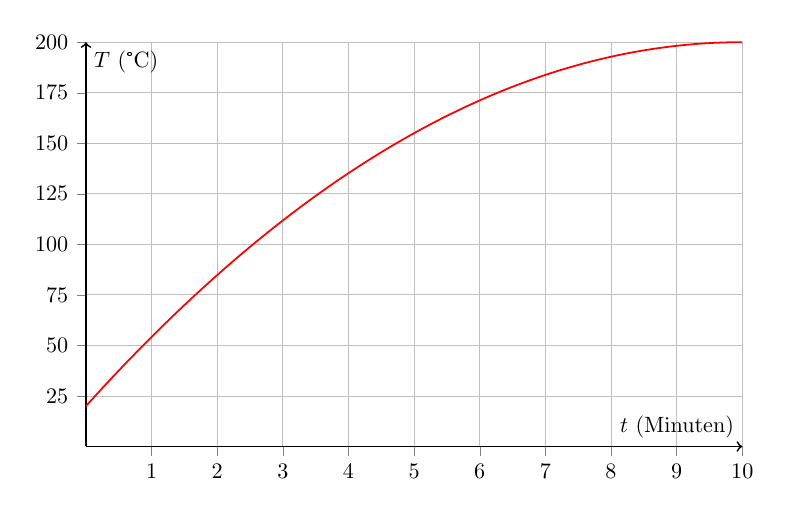
\begin{tikzpicture}[scale=0.8]
        \begin{axis}[
            width=12cm, height=8cm,
            grid=major,
            xlabel={$t$ (Minuten)},
            ylabel={$T$ (°C)},
            xmin=0, xmax=10,
            ymin=0, ymax=200,
            xtick={0,1,2,3,4,5,6,7,8,9,10},
            ytick={0,25,50,75,100,125,150,175,200},
            domain=0:10,
            samples=100,
            thick,
            smooth,
            axis lines=middle,
            axis line style={->},
            enlargelimits=false,
            clip=false,
            tick align=outside
        ]
        \addplot[red, thick] {-9/5*(x-10)^2 + 200};
        \end{axis}
    \end{tikzpicture}
\end{center}
\begin{enumerate}
    \item Berechne die Steigung der Sekante, welche den Graphen von $T$ an den Stellen $t_1=5$ und $t_2=7$ schneidet.
    \item Was hat das Resultat aus 1. für eine Einheit? Was für eine Bedeutung hat es in Bezug auf den Ofen?
    \item \textbf{Challenge:} Gib einen Term in Abhängigkeit von $\Delta t$ an, mit dem man die Steigung der Sekante berechnen kann, die den Graphen von $T$ an den Stellen $t_1=5$ und $t_2=5+\Delta t$ schneidet.
    \item \textbf{Challenge:} Was passiert, wenn $\Delta t$ immer kleiner wird ($\Delta t \to 0$)? Was für eine geometrische und physikalische Bedeutung hat der Grenzwert?
\end{enumerate}

\end{LA}



























\clearpage
\subsection{Differenzenquotient und Differentialquotient}
Die Lernaufgaben zu Beginn des Abschnittes beschreiben gänzlich unterschiedliche Situationen. Die Rechenschritte, die zur Antwort auf die gestellten Fragen geführt haben, weisen aber enorme Parallelen auf. Damit wir diese Gemeinsamkeiten unabhängig vom gewählten Kontext hervorheben können, werden wir sie im Folgenden an einer generischen Funktion $f$ beschreiben.
 Betrachten wir also eine Funktion $f$, die auf einem Intervall der reellen Zahlen definiert ist:


\begin{definition}
    {Differenzenquotient}{}
    Zu einer gegebenen Funktion und zwei verschiedenen Stellen $x_0$ und $x_0+\Delta x$ heisst der Term:
\[
    \frac{f(x_0+\Delta x)-f(x_0 )}{\Delta x}
\]
Differenzenquotient.

Er gibt die Steigung der Sekante durch die Punkte \((x_0, f(x_0))\) und \((x_0+\Delta x, f(x_0+\Delta x))\) an.

\begin{center}
    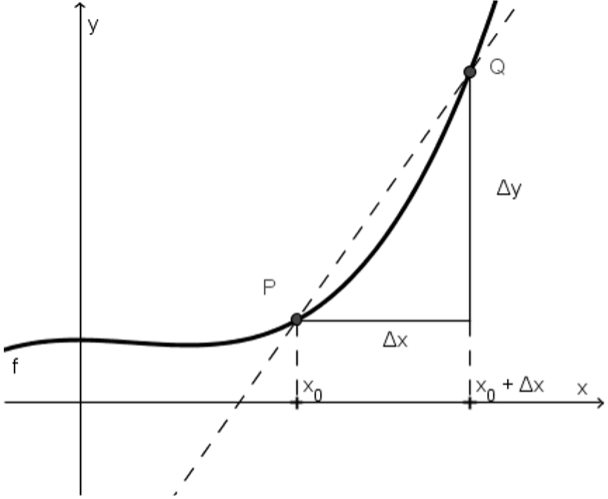
\includegraphics[width = 0.5 \textwidth]{media/differenzenquo.png}
 \end{center}


Häufig wird statt $\Delta x$ auch der Buchstabe $h$ (für horizontaler Abstand) verwendet. Der Differenzenquotient lautet dann:
\[
    \frac{f(x_0+h)-f(x_0 )}{h}
\]


\end{definition}

Je nach Anwendung kann der Differenzenquotient die \emph{durchschnittliche} Geschwindigkeit einer Sprinterin, die \emph{durchschnittliche} Beschleunigung einer Rakete oder die \emph{durchschnittliche} Abnahmerate der Wirkstoffkonzentration pro Zeiteinheit eines Medikaments darstellen.

Ist man an der \emph{momentanen} Geschwindigkeit, Beschleunigung oder Änderungsrate interessiert, bedient man sich einer Methode, die wir in den Einführungsaufgaben mehrfach angewendet haben: Wir lassen $\Delta x$ bzw. $h$ immer kleiner werden und untersuchen das Grenzverhalten des Differenzenquotienten für $\Delta x\to 0$ bzw. $h\to 0$.

\begin{definition}{Differentialquotient}{}
    Falls der Grenzwert
    \[
    \lim\limits_{h\to 0} \frac{f(x_0+h)-f(x_0 )}{h}
    \]
    existiert, so nennt man ihn Differentialquotient oder (erste) Ableitung der Funktion an der Stelle $x_0$. 
    \begin{center}
        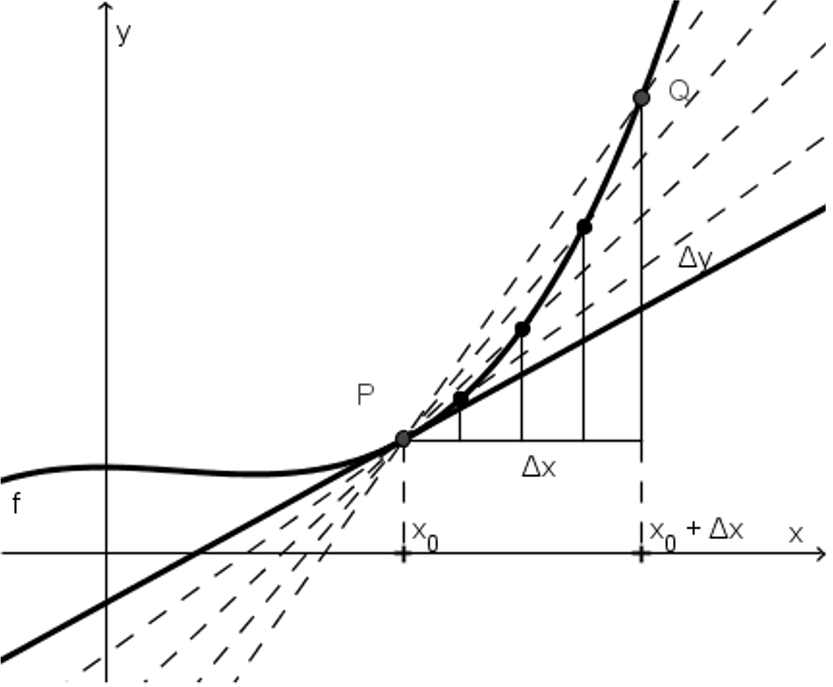
\includegraphics[width = 0.5 \textwidth]{media/differentialquo.png}
     \end{center}
    
    Bezeichnungen:
    \[
        f'(x_0) \quad \text{oder} \quad \frac{d}{dx} f(x_0)
    \]
    Gesprochen: „$f$ Strich von $x_0$“ oder „$df$ nach $dx$ an der Stelle $x_0$“.
    
    Die Ableitung der Funktion an der Stelle $x_0$ entspricht der Steigung der Tangente an den Graphen im Punkt $ (x_0, f(x_0)) $.  
    
    
    
\end{definition}


\begin{bsp}
    {Berechnung des Differentialquotienten}{}
    Gegeben sei die Funktion $f(x)=\frac{1}{2}x^2-x$. Gesucht ist die Ableitung von $f$ an der Stelle $x_0=5$

    \vspace*{6.5cm}

    % Als erstes bestimmen wir den Differenzenquotienten:
    % \begin{align*}
    %    \frac{\Delta y}{\Delta x} &= \frac{f(5+h)-f(5)}{h} \\
    %    &= \frac{\left(\frac{1}{2} (5+h)^2-(5+h) \right) - \left(\frac{1}{2}5^2 -5 \right)}{h} \\
    %    %&= \frac{\left(\frac{1}{2}(25+10h+h^2)\right)-\frac{15}{2}}{h} //
    %    &= \frac{\frac{1}{2}h^2+4h}{h}
    % \end{align*}
    % Anschliessend bilden wir den Grenzwert für $h\rightarrow0$:
    % $$f'(5) = \lim_{h\rightarrow0}\frac{\Delta y}{\Delta x}= \lim_{h\rightarrow0} \frac{\frac{1}{2}h^2+4h}{h} = \lim_{h\rightarrow0}\left(\frac{1}{2}h+4\right) = 4$$
\end{bsp}


\begin{ueb}
    {}{}
    \begin{enumerate}
        \item Skizziere den Graphen der Funktion \( f(x) = 2x^2 \). Beantworte dann die folgenden Fragen mit einer Rechnung:
        \begin{enumerate}
          \item  Welche Steigung hat die Sekante, welche den Graphen an den Stellen \( x = 1 \) und \( x = 2 \) schneidet?
          \item Welche Steigung hat die Sekante, welche den Graphen an den Stellen \( x = 1 \) und \( x = 1 + h \) schneidet?
          \item Welche Steigung hat die Tangente, die den Graphen an der Stelle \( x = 1 \) berührt?
          \item Welche Steigung hat jene Tangente, die den Graphen an der Stelle \( x = 2 \) berührt?
        \end{enumerate}
      
        \item Sei \( f(x) = x^3 \).
       Berechne \( f'(2) \).
      
        \item Skizziere den Graphen der Funktion \( f(x) = x^2 - 5 \).
        \begin{enumerate}
          \item Berechne \( f'(0) \). Welche Eigenschaft des Graphen wird durch das Resultat verdeutlicht?
          \item Berechne \( f'(2) \). 
          \item Bestimme \( f'(-2) \). Entweder mit dem Differentialquotient oder indem du eine Eigenschaft der Parabel verwendest\dots
        \end{enumerate}
      
        \item Zeichne den Graphen der Funktion \( f(x) = \frac{1}{3}x - 1 \).\\
              Entscheide ohne zu rechnen: Wie gross sind \( \frac{d}{dx} f(1) \), \( \frac{d}{dx} f(2) \) und \( \frac{d}{dx} f(-42) \)?
        
        \item Die Funktion $N(t)$ beschreibt die Anzahl Bakterien einer Bakterienkultur $t$ Tage nach Beginn des Experiments. Beschreibe die Bedeutung der folgenden Grössen und geben deren Einheit an.
        \begin{enumerate}
            \item $N(10)-N(5)$
            \item $\frac{N(10)-N(5)}{5}$
            \item $\lim\limits_{h\to0}\frac{N(5+h)-N(5)}{h}$
        \end{enumerate}

        \item Ein Teilchen bewegt sich mit der Geschwindigkeit $v(t) = 2t^2 - 5t + 1$ [m/s] in Abhängigkeit von der Zeit $t$ [s]. Berechne die momentane Beschleunigung des Teilchens zum Zeitpunkt $t=1$.
        
        Bestimmen Sie auch die momentane Geschwindigkeit zur Zeit $t=1$ und beschreiben Sie die Bewegung des Teilchens zu diesem Zeitpunkt.
      
        \item \textbf{Achtung Doppelbrüche!}\\
        Sei \( f(x) = \frac{1}{x + 1} \). Berechne \( f'(1) \).
    
      \end{enumerate}
\end{ueb}

\clearpage
\emph{Lösungen:}


\begin{enumerate}
  \item
  \begin{enumerate}
    \item \( 6 \)
    \item \( 4 + 2h \)
    \item \( 4 \)
    \item \( 8 \)
  \end{enumerate}

  \item
   \( 12 \)
  

  \item
  \begin{enumerate}
    \item \( f'(0) = 0 \)
    \item \( f'(2) = 4 \)
    \item  \( f'(-2) = -4 \)
  \end{enumerate}

  \item
  \[
  \frac{d}{dx}f(1) = \frac{1}{3}, \quad
  \frac{d}{dx}f(2) = \frac{1}{3}, \quad
  \frac{d}{dx}f(-42) = \frac{1}{3}
  \]
  \item 
        \begin{enumerate}
            \item Bevölkerungszuwachs in Anzahl Bakterien.
            \item \emph{Durchschnittliche} Wachstumsrate der Population zwischen dem 5 und 10 Tag in Bakterien/Tag.
            \item  \emph{Momentane} Wachstumsrate der Population am fünften Tag in Bakterien/Tag.
        \end{enumerate}
\item Beschleunigung des Teilchens am Zeitpunkt \( t=1 \):
\[
    a(1) = v'(1) = -1
\]
Ausserdem gilt $v(1)=-2$. Bezüglich der ausgelegten Skala, welche die Position des Teilchens beschreibt, bewegt sich das Teilchen so, dass die Werte abnehmen. Wegen der negativen Beschleunigung, bewegt sich das Teilchen immer schneller in negativer Richtung.
  \item
   \( f'(1) = -\frac{1}{4} \)
  
\end{enumerate}
























\clearpage
\subsection{Ableitungsfunktion}




Nach den Erkenntnissen aus dem Kapitel über Grenzwerte wissen wir, dass diese nicht immer existieren. Somit kann es auch sein, dass für eine gegebene Funktion den Differentialquotienten an einer bestimmten Stelle gar nicht gebildet werden kann.
\begin{definition}
    {Differenzierbarkeit}{}
    Sei $f$ eine beliebige Funktion und $x_0 \in \mathbb{D}_f$. Falls der Grenzwert 
    $$ \lim_{h\rightarrow0}\frac{f(x_0+h)-f(x_0)}{h} $$
    existiert, so sagt man, dass die Funktion $f$ an der Stelle $x_0$ \emph{differenzierbar} ist.
\end{definition}

Die Betragsfunktion $x\mapsto |x|$ ist beispielsweise überall differenzierbar mit Ausnahme der Stelle $x_0=0$.

\begin{center}
    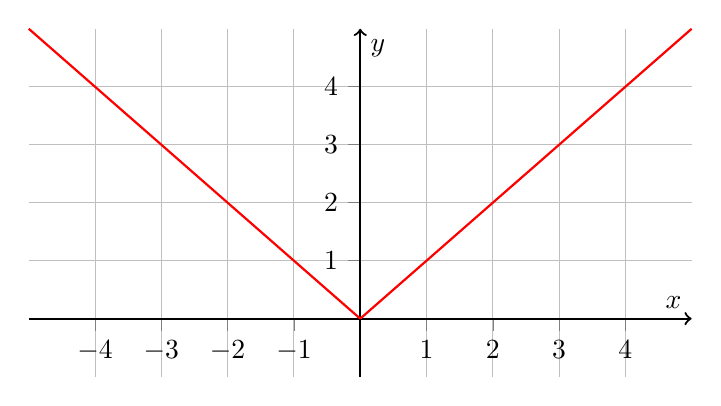
\begin{tikzpicture}
        \begin{axis}[
            width=10cm, height=6cm,
            grid=major,
            xlabel={$x$},
            ylabel={$y$},
            xmin=-5, xmax=5,
            ymin=-1, ymax=5,
            xtick={  -4, -3, -2, -1, 0,1,2,3,4},
            ytick={0,1,2,3,4},
            domain=-5:5,
            samples=500,
            thick,
            smooth,
            axis lines=middle,
            axis line style={->},
            enlargelimits=false,
            clip=false,
            tick align=outside
        ]
        \addplot[red, thick] {abs(x)};
        \end{axis}
    \end{tikzpicture}
\end{center}


% \begin{center}
%     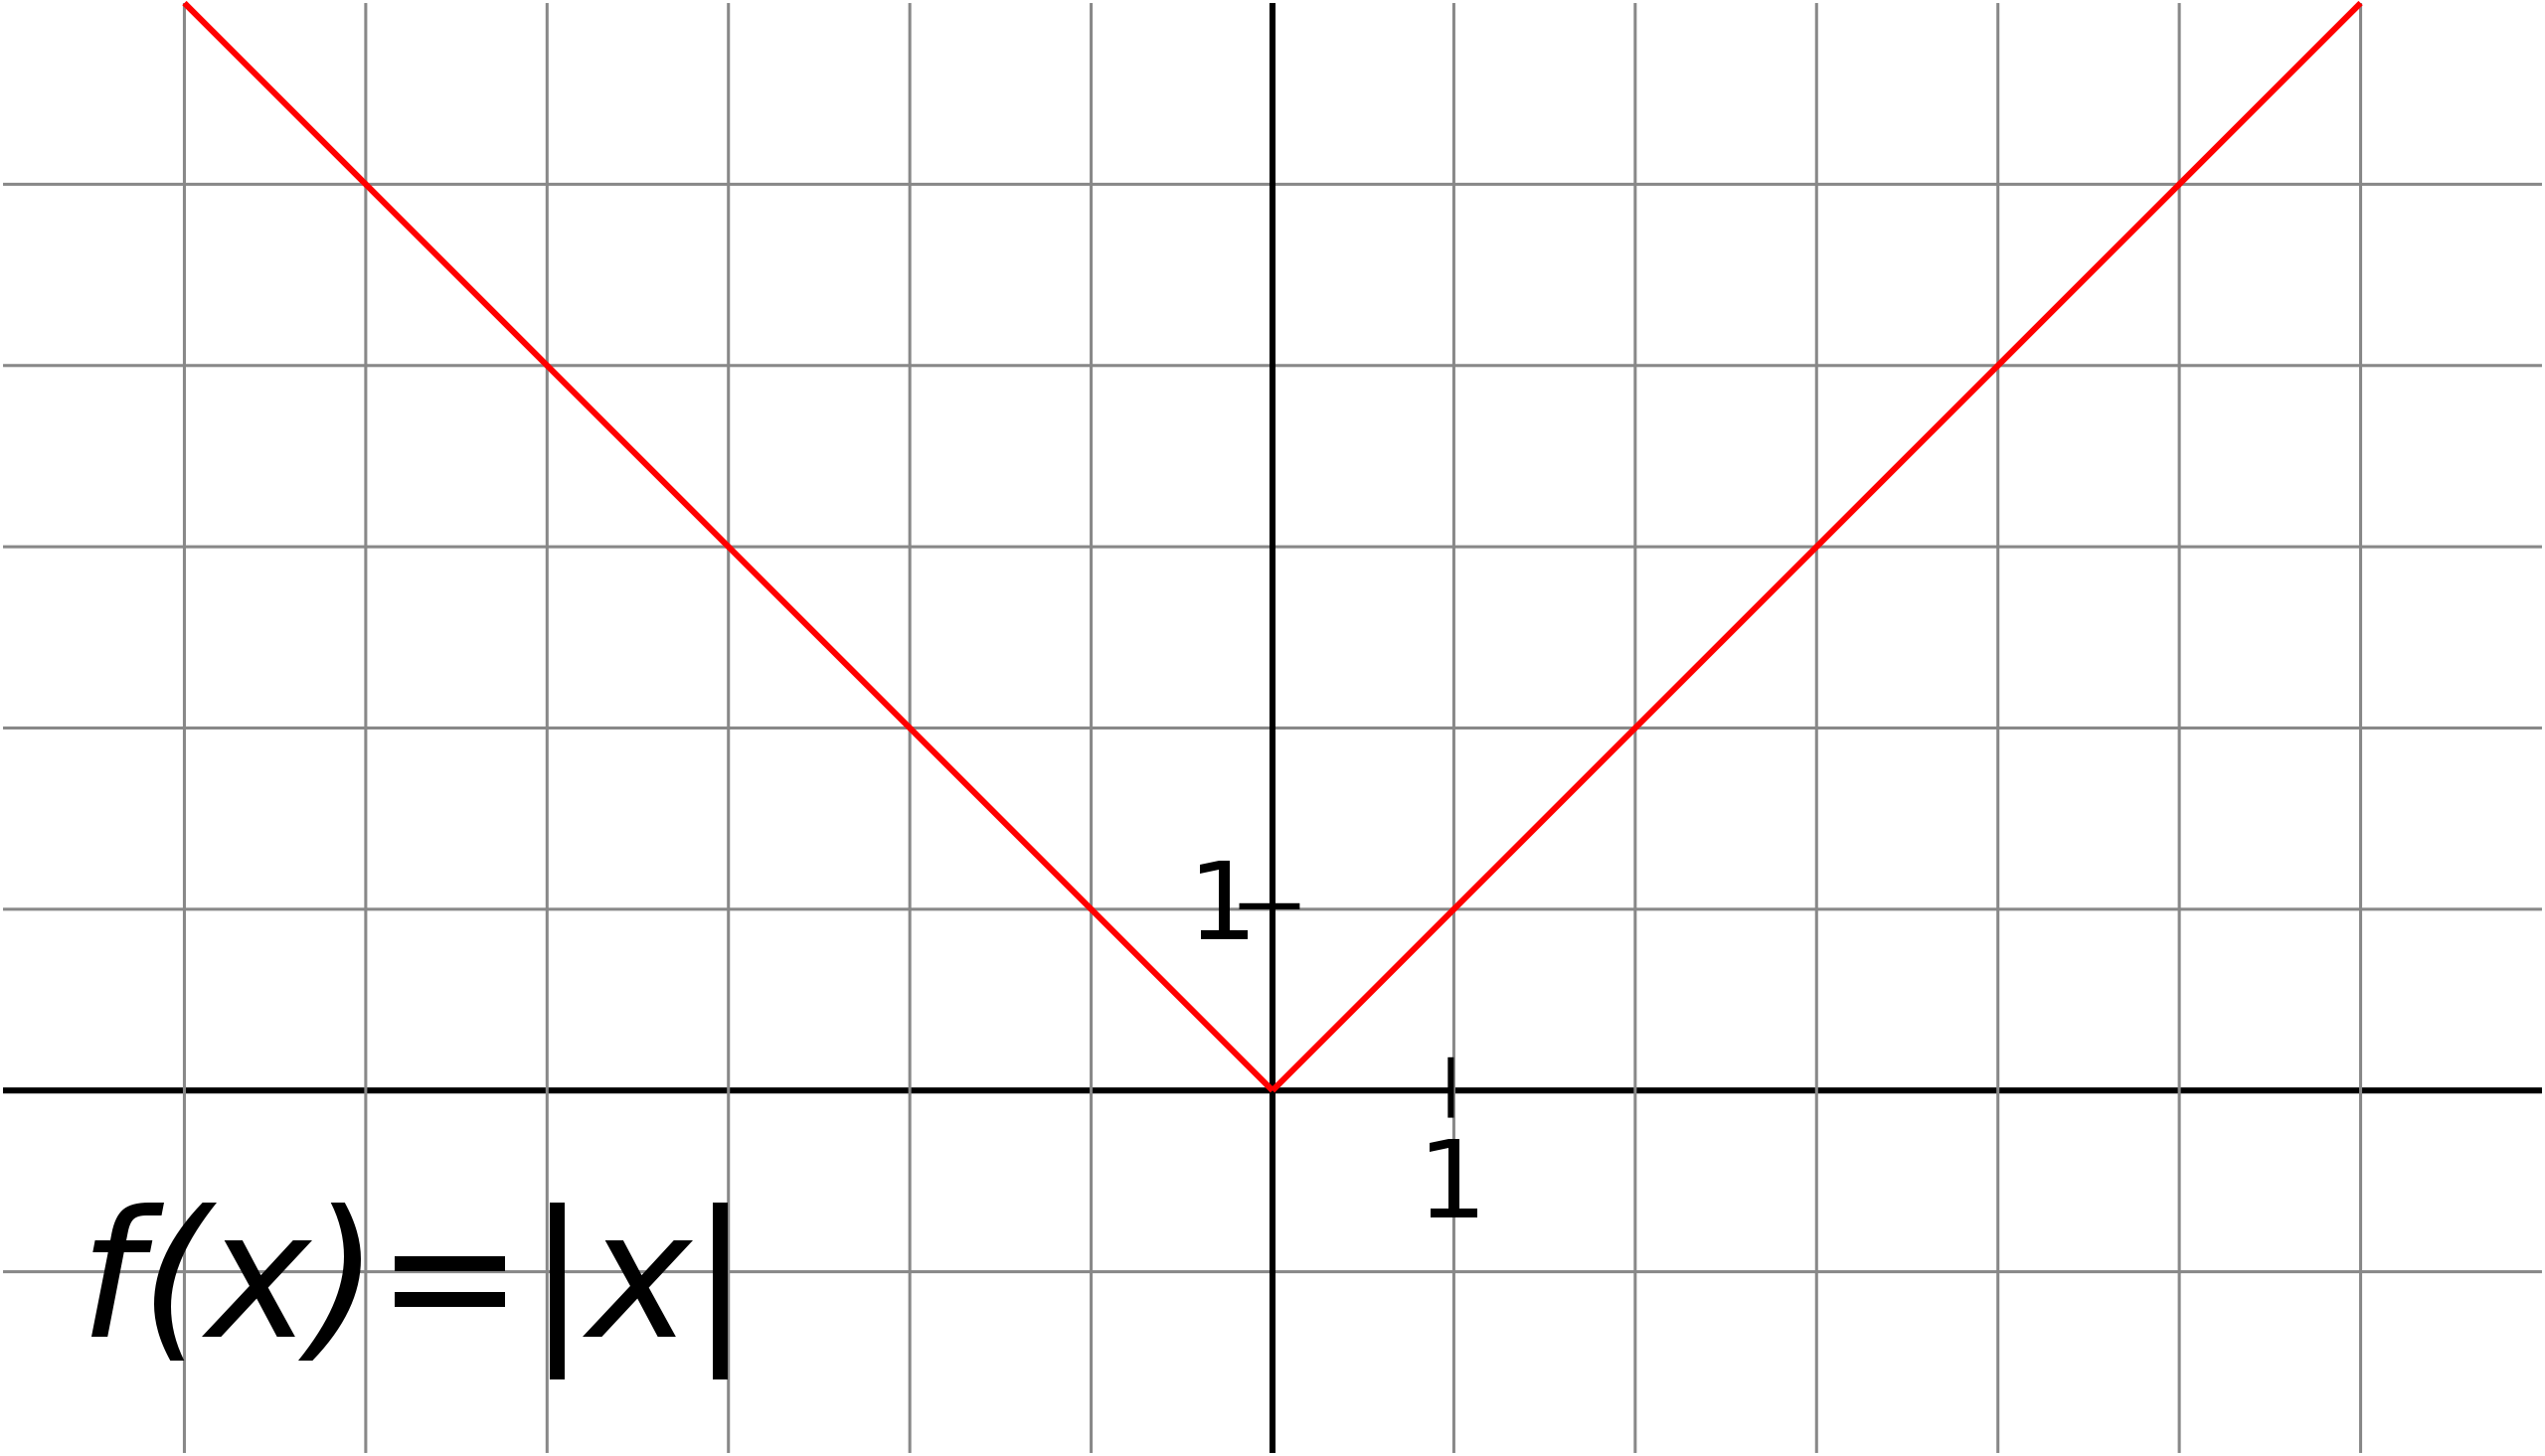
\includegraphics[scale=0.1]{media/Abs(x).png}
% \end{center}
Was wären in diesem Fall der links- bzw. rechtsseitige Grenzwert $\lim\limits_{h\nearrow 0} \frac{f(0+h)-f(0)}{h}$ und $\lim\limits_{h\searrow 0} \frac{f(0+h)-f(0)}{h}$?

Wenn die Funktion überall differenzierbar ist, kann in jedem Punkt des Graphen die Steigung der Tangente ermittelt werden. Die Zuordnung \emph{
$x\mapsto$ Steigung des Graphen von $f$ an der Stelle $x$} ist wieder eine Funktion!

\begin{definition}
    {Ableitungsfunktion}{}
    Gegeben sei eine differenzierbare Funktion $f$. Die Funktion mit der Zuordnungsvorschrift:
    $$x\mapsto f'(x)=\lim_{h\rightarrow0}\frac{f(x+h)-f(x)}{h}$$
    heisst die \emph{Ableitungsfunktion} (kurz: \emph{die Ableitung}) der Funktion $f$. Sie wird mit $f'$ bezeichnet. 
    \newline
    Geometrisch interpretiert beschreibt der Output von $f'$ die Steigung der Tangente an den Graphen von $f$ im Punkt $(x|f(x))$.
  
\end{definition}

Einen ungefähren Verlauf der Ableitungsfunktion kann man sich mit rein grafischen Überlegungen machen:
\begin{bsp}{Graph der Ableitungsfunktion}{}
    In der folgenden Abbildung ist der Graph einer Funktion $f$ dargestellt. Skizziere den ungefähren Verlauf des Graphen der Ableitungsfunktion $f'$.
    \begin{center}
        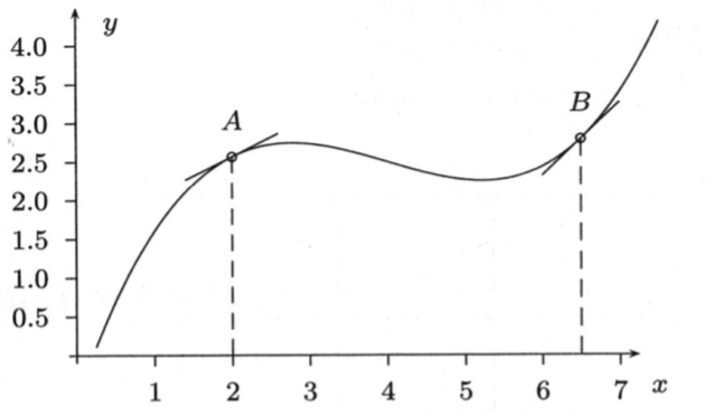
\includegraphics[scale = 1.2]{media/graphischesAbleiten.png}
    \end{center}
    \vspace{12
    cm}
\end{bsp}

\clearpage
\begin{ueb}
    {Graph der Ableitungsfunktion}{}
    \begin{enumerate}
        \item Die Grafiken I bis IV zeigen die ursprünglichen Graphen von vier Funktionen $f$, die Grafiken a) bis d) die Graphen der vier Ableitungsfunktionen $f'$. Welcher $f$-Graph gehört zu welchem $f'$-Graph?
        \begin{center}
            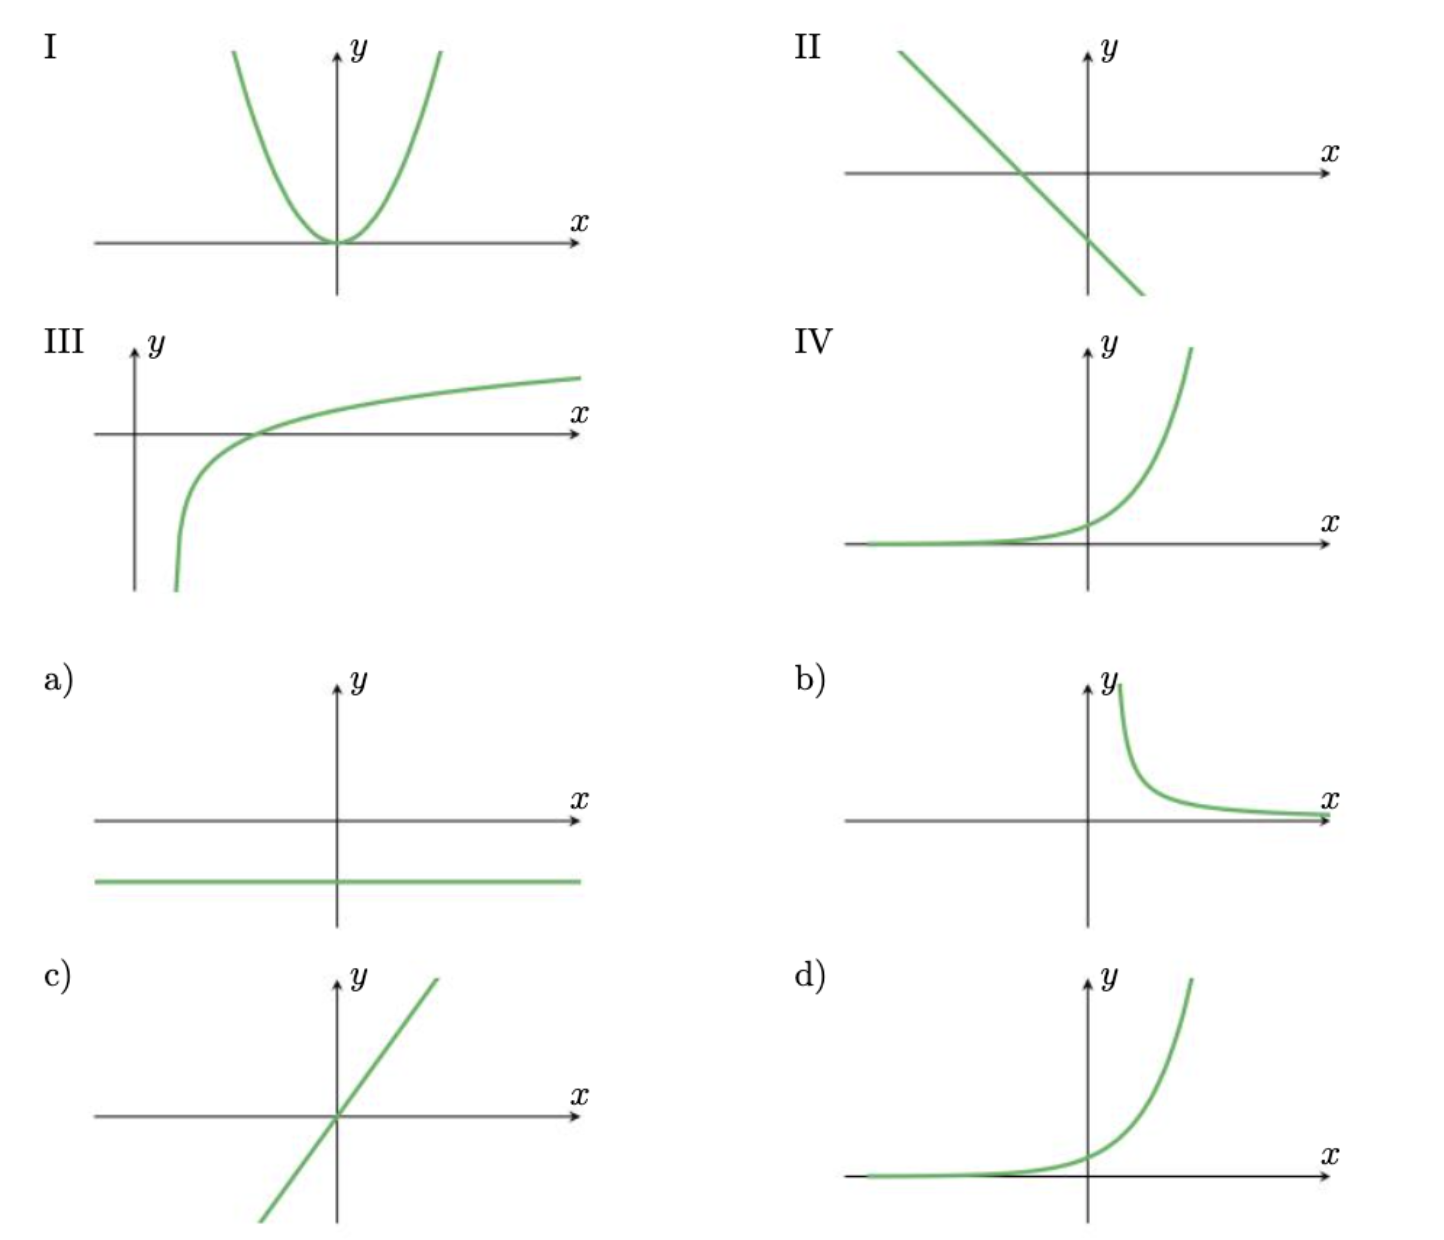
\includegraphics[width = 0.8 \textwidth]{media/zuordnungf-f.png}
        \end{center}
        \item Skizziere den Graphen der Ableitungsfunktion $f'$ der dargestellten Funktion $f$ in das gleiche Koordinatensystem.
        \begin{center}
            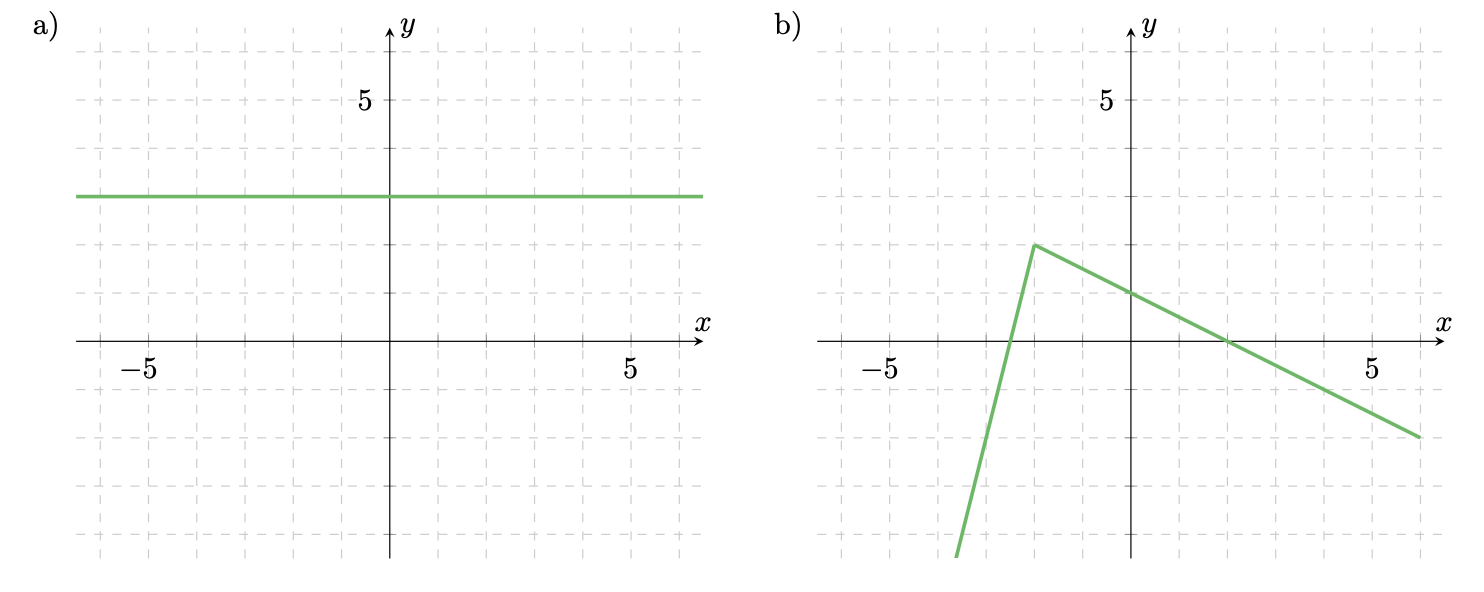
\includegraphics[width = 0.8 \textwidth]{media/graphischAbleiten1.png}
        \end{center}
        \pagebreak
        \item Skizziere den Graphen der Ableitungsfunktion $f'$ der dargestellten Funktion $f$ in das gleiche Koordinatensystem.
        \begin{center}
            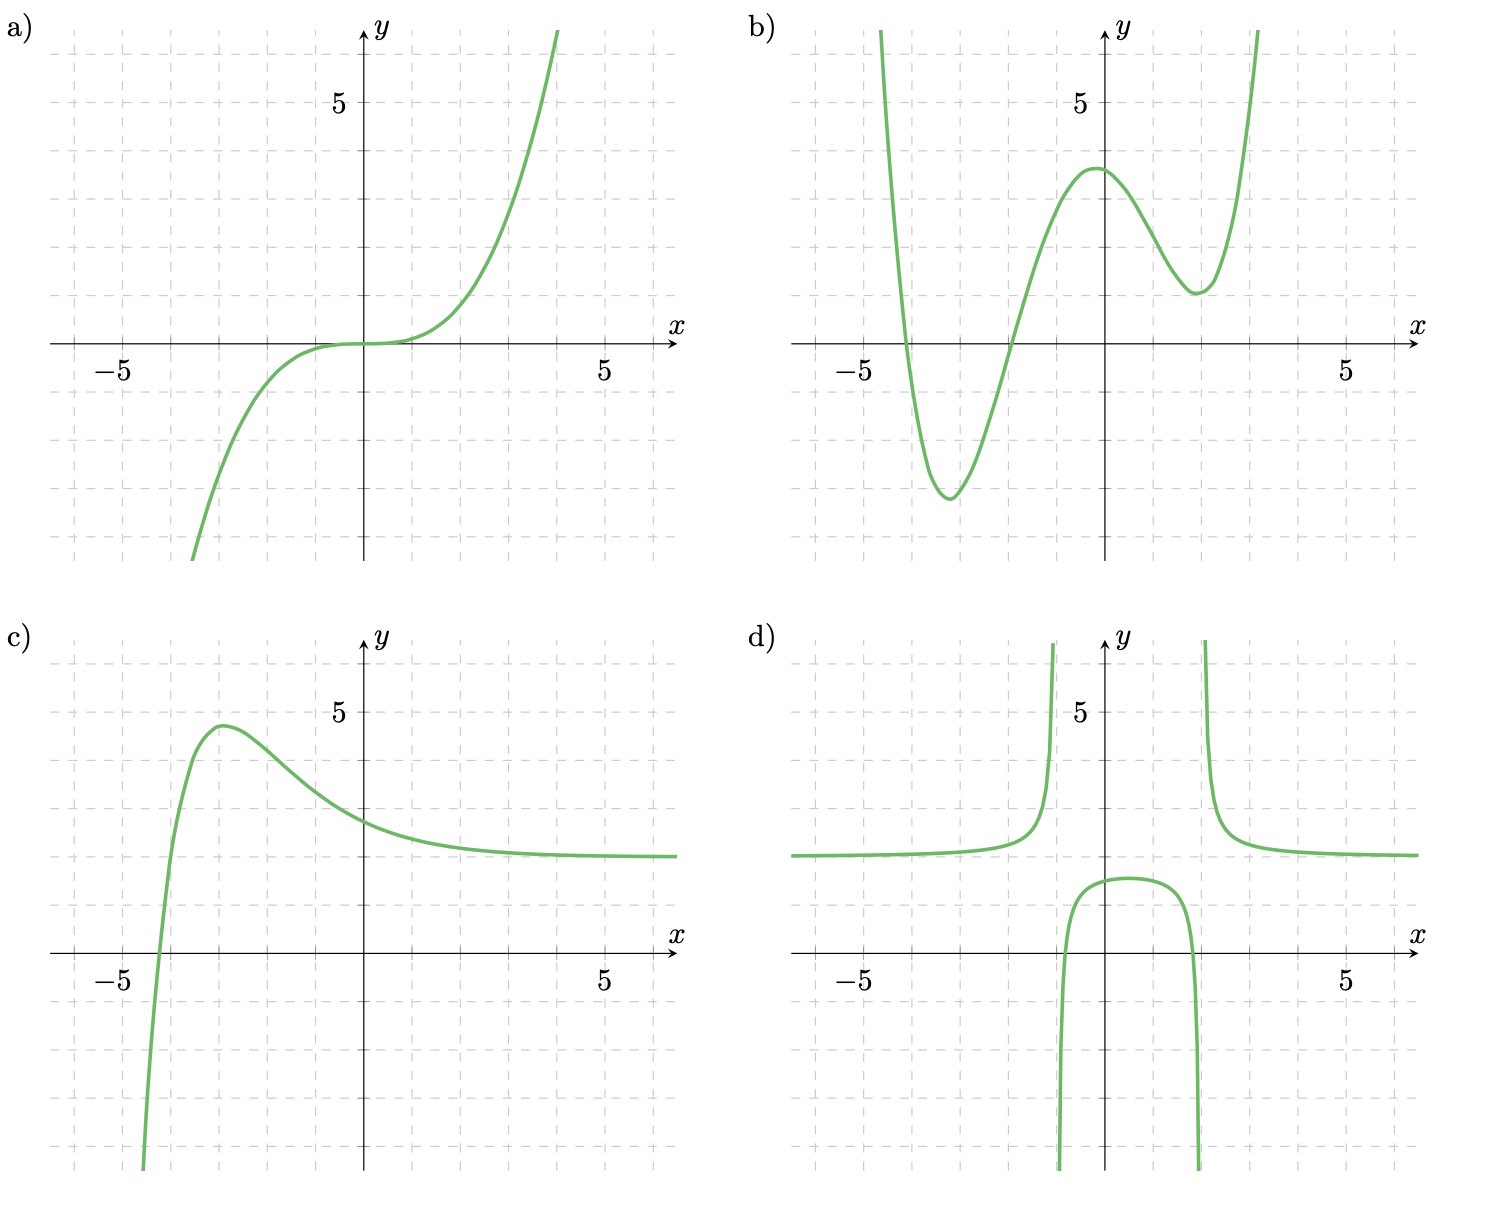
\includegraphics[width = 0.8 \textwidth]{media/GraphischAbleiten 2.png}
        \end{center}
    \end{enumerate}
\end{ueb}

\clearpage
\emph{Lösungen:}
\begin{enumerate}
    \item I-c), II-a), III-b), IV-d)
    \item Ableitungsgraphen
    
    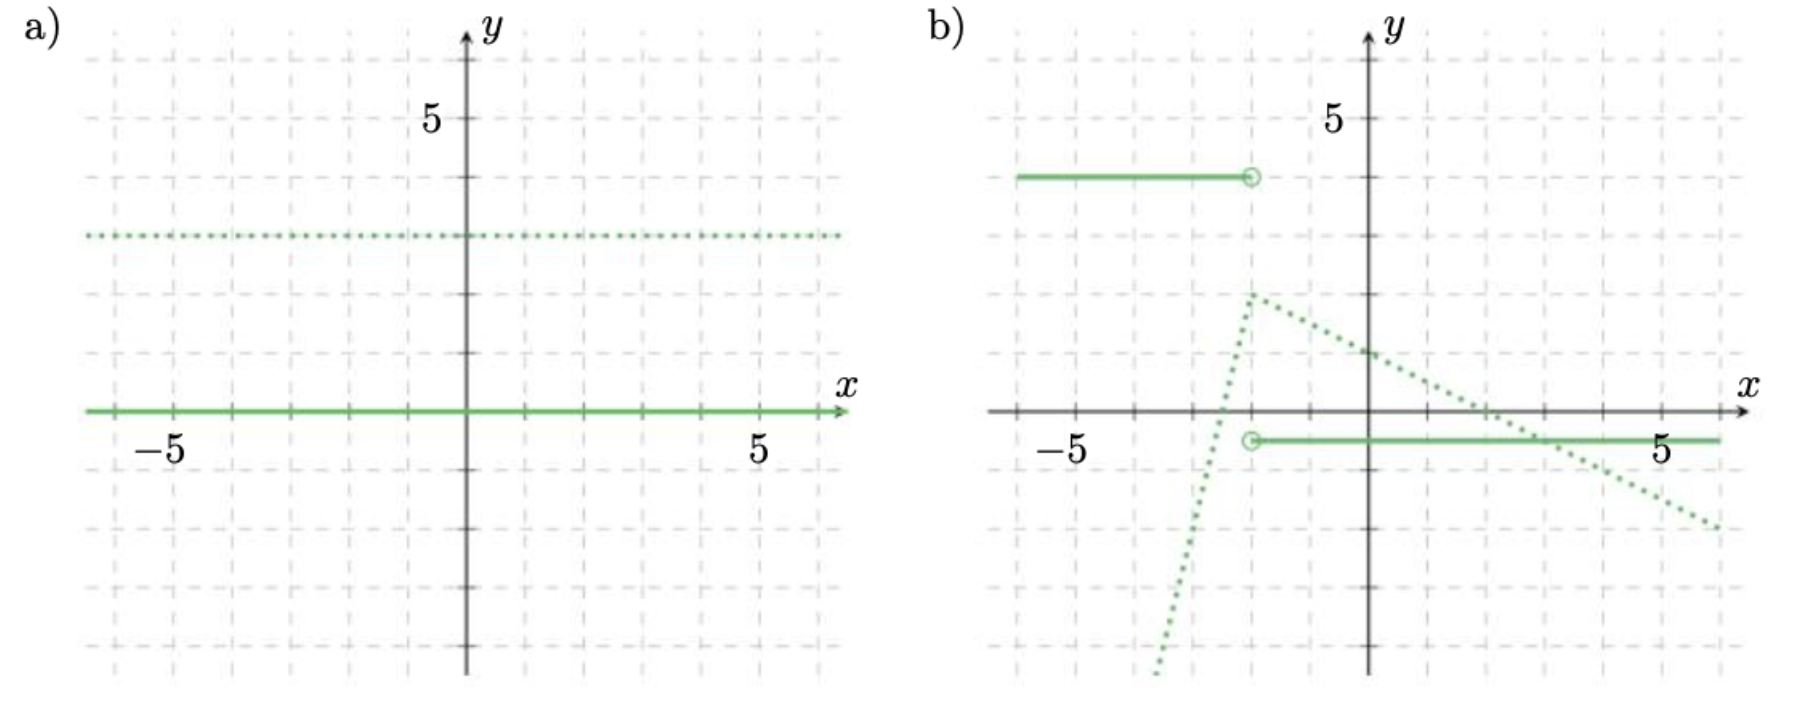
\includegraphics[width = 0.8 \textwidth]{media/lsgGraphischAbleiten1.png}
    
    \item Ableitungsgraphen
    
    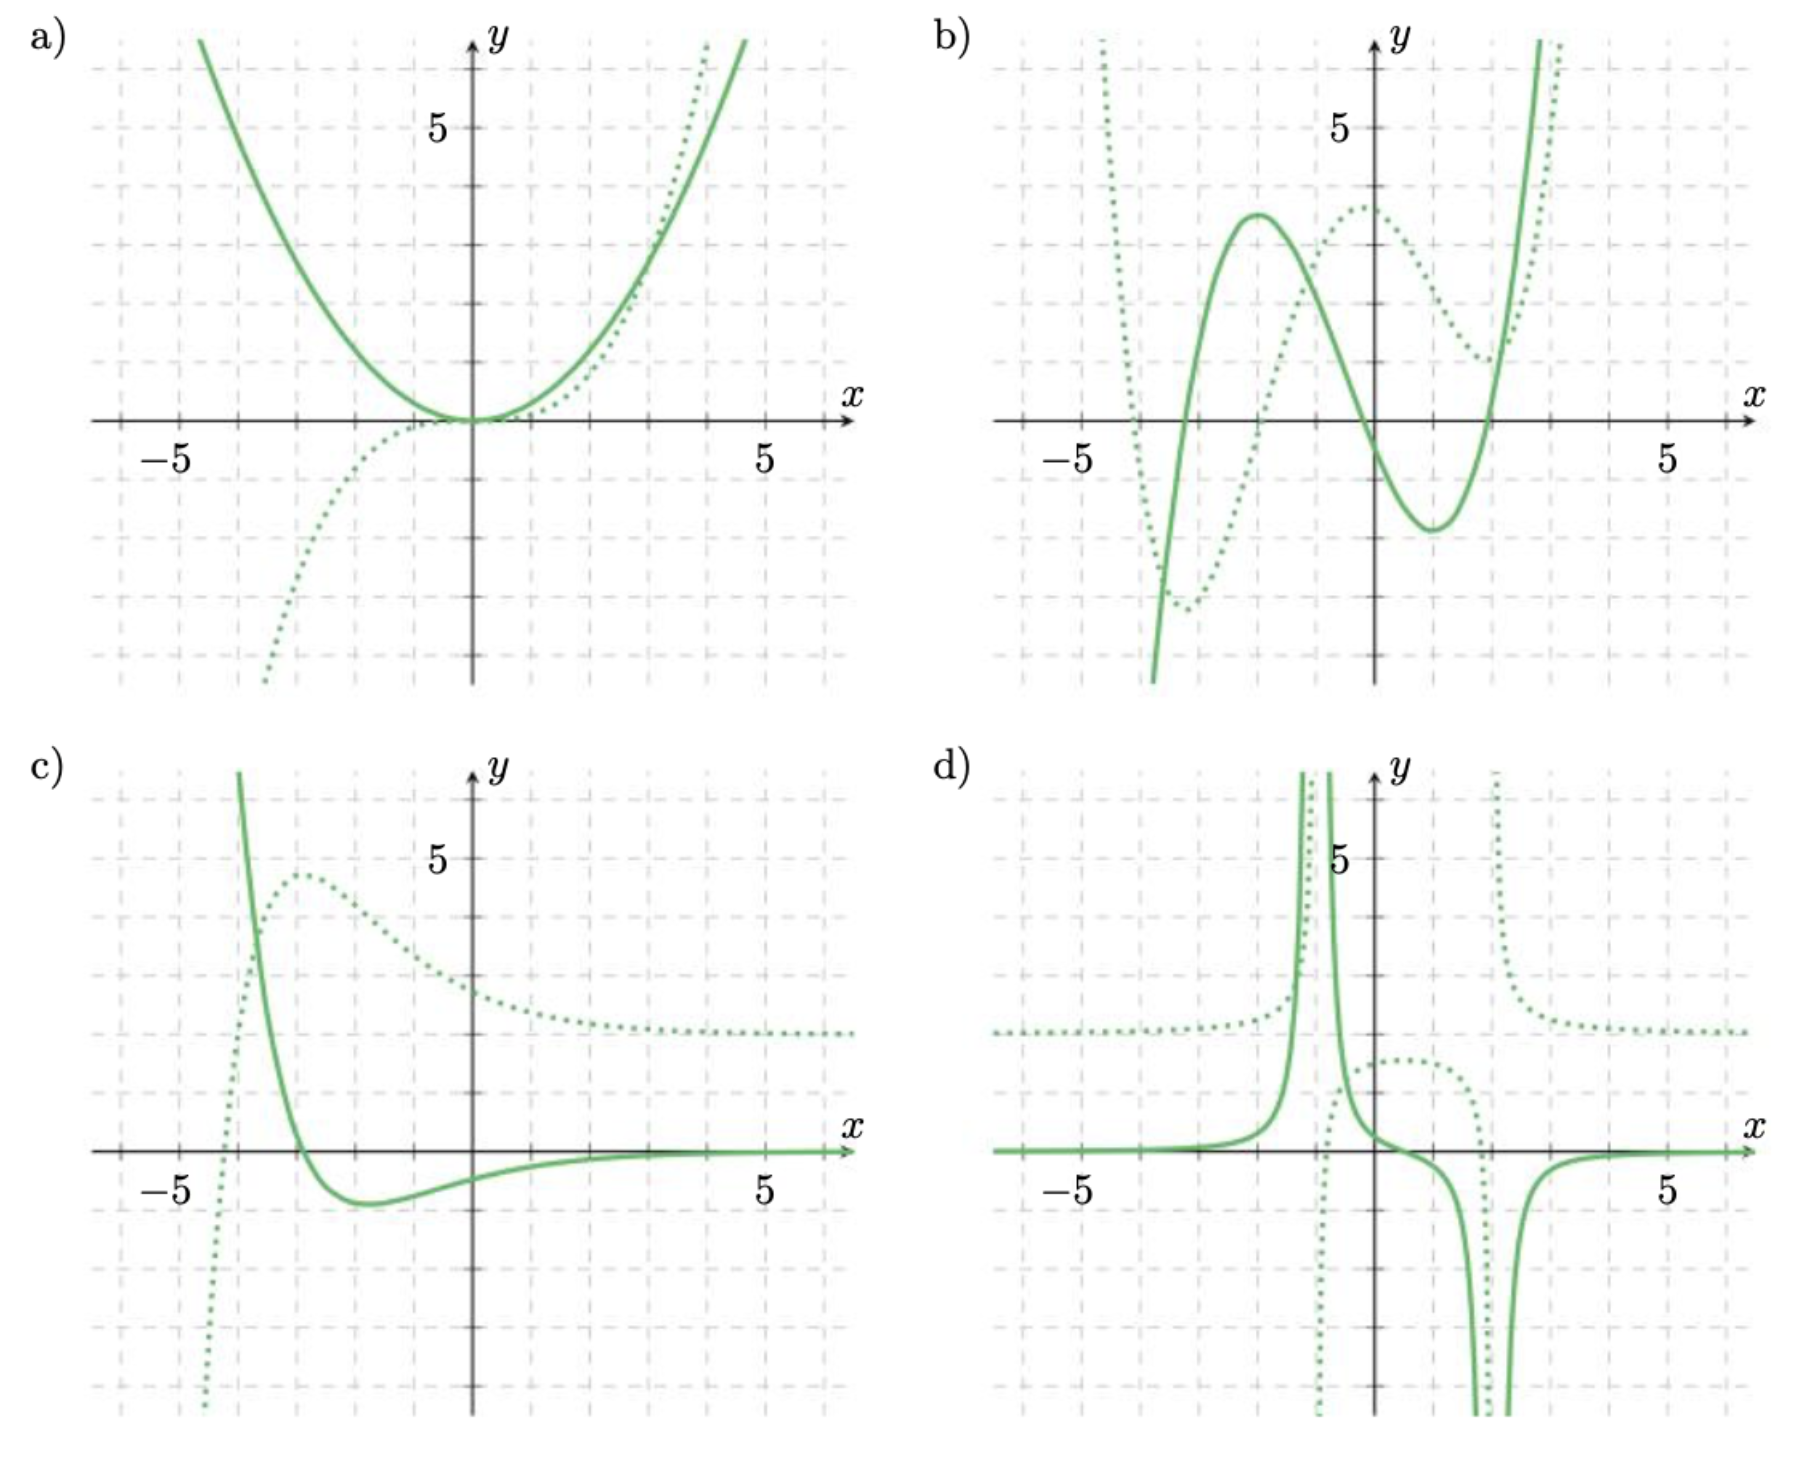
\includegraphics[width = 0.8 \textwidth]{media/LsgGraphischAbleiten2.png}

\end{enumerate}


















\clearpage
Häufig möchte man auch die Funktionsgleichung der Ableitung ermitteln, nicht nur den ungefähren Verlauf des Graphen. Dazu greift man wieder zum Differenzialquotienten. 
$$f'(x) = \lim_{h\to0}\frac{f(x+h)-f(x)}{h}$$

Betrachten wir dazu ein Beispiel:

\begin{bsp}
    {Berechnung der Ableitungsfunktion}{berechnenderAbleitung}
    Sei $f(x)=x^2+1$. Die Gleichung der Ableitungsfunktion kann wie folgt hergeleitet werden:

    \vspace*{15cm}
    % \begin{align*}
    %     f'(x)   &= \lim_{h\rightarrow0}\frac{f(x+h)-f(x)}{h}\\
    %             &=  \lim_{h\rightarrow0}\frac{\left((x+h)^2+1\right)-\left(x^2+1\right)}{h}\\
    %             &= \lim_{h\rightarrow0}\frac{\left(x^2+2hx+h^2+1\right)-\left(x^2+1\right)}{h}\\
    %             &= \lim_{h\rightarrow0}\frac{2hx+h^2}{h}\\
    %             &= \lim_{h\rightarrow0}\left(2x+h\right)\\
    %             &= 2x
    % \end{align*}
    % Die erste Ableitung von $f$ ist damit $f'(x)=2x$. In anderen Worten: Die Tangente, welche den Graphen von $y=x^2+1$ an der Stelle $x$ berührt hat die Steigung $2x$.
    % So hat die Tangente an $y=x^2+1$ an der Stelle $x=5$ die Steigung $f'(5)=10$.
    
\end{bsp}
\clearpage
Mit der Gleichung der Ableitungsfunktion lässt sich die Geradengleichung der Tangente an einen Funktionsgraphen bestimmen:

\begin{bsp}
    {Gleichung der Tangente}{}
    Sei wieder $f(x)=x^2+1$. Wie lautet die Gleichung der Tangente, welche den Graphen an der Stelle $x=5$ berührt?
    
    \vspace*{18cm}

\end{bsp}

\clearpage
\begin{ueb}
    {}{}
    \begin{enumerate}
        \item 
    Bestimme die Gleichung der Ableitungsfunktion \( f' \) der Funktion \( f  \).

            \begin{enumerate}
            \item \( f(x) = x^2 + 3 \). Vergleiche das Resultat mit \Cref{bsp:berechnenderAbleitung} und erkläre.
            \item \( f(x) = 2x^3 \). Verwende das Pascalsche Dreieck.
            \item \( f(x) = 3x \). Wieso ergibt das seltsame Resultat Sinn?
            \item \( f(x)= \dfrac{1}{x} \). Achtung Doppelbrüche!
            \item \( f(x) =\sqrt{x} \). Tipp: Erweitere den Differenzenquotienten mit $\sqrt{x+h} + \sqrt{x}$ 
            \end{enumerate}
    \item Bestimme die Gleichung der Tangente, welche die Funktion $f$ an der Stelle $x_0$ berührt. Verwende die Resultate aus Aufgabe 1.
    \begin{enumerate}
        \item \( f(x) = x^2 + 3, \qquad x_0  = -3 \). 
        \item \( f(x) = 2x^3 , \qquad x_0  = 1 \).
        \item \( f(x) = 3x , \qquad x_0  = 1 \). 
        \item \( f(x)= \dfrac{1}{x} , \qquad x_0  = 2 \). 
        \item \( f(x) =\sqrt{x}, \qquad x_0  = 4 \).
        \end{enumerate}
    % \item Bestimme die Gleichung der Tangente, welche die Funktion $f= x^2 - x$ an der Stelle $x_0=1$ berührt.
    \item Die Position eines Teilchens wird durch die Funktion $s(t) = (2-t)^2$ beschrieben. Bestimmen Sie die Funktion $v(t)$, welche die momentane Geschwindigkeit des Teilchens zum Zeitpunkt $t$ beschreibt.
\end{enumerate}
\end{ueb}

\pagebreak
\emph{Lösungen:}
\begin{enumerate}
    \item Ableitungsfunktionen:
    \begin{enumerate}
      \item \( f'(x) = 2x \)
      \item \( f'(x) = 6x^2 \)
      \item \( f'(x) = 3 \)
      \item \( f'(x) = -\dfrac{1}{x^2} \)
      \item \( f'(x) = \dfrac{1}{2\sqrt{x}} \)
    \end{enumerate}
  
    \item Tangentengleichungen:
    \begin{enumerate}
      \item \( y = -6x - 6 \)
      \item \( y = 6x - 4 \)
      \item \( y = 3x \)
      \item \( y = -\dfrac{1}{4}x + 1 \)
      \item \( y = \dfrac{1}{4}x +1\)
    \end{enumerate}
  
    % \item Tangente an \( f(x) = x^2 - x \) bei \( x_0 = 1 \):
    % \[
    % y = x - 1
    % \]
    \item $v(t) = 2t-4$ 
  \end{enumerate}

